\documentclass[a4paper,12pt]{report}

\usepackage{alltt, fancyvrb, url}
\usepackage{graphicx}
\usepackage[utf8]{inputenc}
\usepackage{float}
\usepackage{hyperref}

% Questo commentalo se vuoi scrivere in inglese.
\usepackage[italian]{babel}

\usepackage[italian]{cleveref}

\title{Relario: Tales of Relano\\Progetto per il corso di\\``Programmazione ad Oggetti''}

\author{Lorenzo Cinelli, Mihai Mazuru, Kimi Osti, Sara Panfini}
\date{\today}


\begin{document}

\maketitle

\tableofcontents

\chapter{Analisi}


\section{Descrizione e requisiti}

Il software realizzato è un videogioco 2D con vista dall’alto. Il suo svolgimento gira attorno a un personaggio principale, controllato dall’utente, che deve attraversare le stanze di un castello per raggiungere lo scontro finale con il Re, di cui deve conquistare il trono.
%
\newline Durante l’esplorazione delle stanze all’utente potranno essere affidate delle quest da completare per poter procedere correttamente.
%
\newline Inoltre, gli verranno presentato delle stanze quasi completamente interattive. In particolare, ci saranno dei personaggi non giocanti (neutri, alleati o nemici) che potranno, al momento dell’interazione, mostrare un messaggio, donare degli oggetti oppure ingaggiare un combattimento. Inoltre, sarà possibile interagire con gran parte degli elementi di arredo presenti in stanza, tra cui elementi come armature o vasi contenenti oggetti collezionabili oppure tappeti o botole che possono celare al loro interno nemici.
%
\newline Il combattimento si svolge per turni. Ad ogni turno, il giocatore può decidere se attaccare o chiedere pietà al nemico, così come può navigare il suo inventario e usare oggetti senza perdere il diritto al turno. Il nemico, in caso venga chiesta pietà, potrebbe concederla oppure rifiutarla e attaccare immediatamente il giocatore. 

\subsubsection{Requisiti funzionali}
\begin{itemize}
	\item I nemici all'interno del gioco saranno di varie tipologie, e dovranno offrire un comportamento variabile all'utente per quanto riguarda le richieste di pietà;
	\item L'arredo delle stanze viene generato casualmente garantendo l'assenza di sovrapposizioni, e le diverse tipologie di elementi di arredo devono offrire diversi scenari di interazione;
	\item Le quest devono essere di diverse tipologie e richiedere diverse azioni da parte del giocatore;
	\item Il combattimento finale deve poter offrire una scelta al giocatore, che sarà in grado di avviare finali diversi.
\end{itemize}

\subsubsection{Requisiti non funzionali}
\begin{itemize}
	\item Per offire un'esperienza gradevole all'utente, si mira a realizzare un software efficiente.
	\item Il software sarà portabile su tutti i maggiori sistemi operativi.
\end{itemize}


\section{Modello del Dominio}

Il dominio applicativo dell’applicazione viene modellato in ogni momento dal concetto di stanza, ovvero il “container” all’interno di cui si svolge la fase centrale del gioco. All’interno della stanza, oltre al personaggio principale, si trovano altre entità, che possono essere personaggi viventi non giocanti (nemici o generici NPC) oppure elementi di arredo. Il giocatore può possedere nel suo inventario diversi oggetti, che vengono anch’essi modellati come entità. In questo scenario, diventa possibile gestire tramite la stanza e le informazioni che ogni entità offre l’intero modello del dominio, estraendo le istanze di interesse per gestire le situazioni contingenti come il combattimento. 
%
\newline Per quanto riguarda l’arredamento, le entità si dividono in tre tipologie fondamentali: arredamento interattivo, che blocca il movimento ma permette interazione, e può rilasciare un oggetto che il giocatore aggiungerà al proprio inventario al momento dell’interazione; arredamento calpestabile, che non ostruisce il movimento e permette interazione, ma può nascondere un nemico con cui viene avviato il combattimento non appena vi si interagisce; arredamento passivo, che ostacola il movimento e non permette alcun tipo di interazione. 
%
\newline Per quanto riguarda i nemici, ad ognuno viene associato un tipo, che ne definisce il livello di difficoltà. Quando viene sconfitto, un nemico rilascia un oggetto di inventario che il giocatore aggiungerà al proprio inventario al momento della vittoria. Ad ogni nemico viene poi associato un comportamento in caso di richieste di pietà, indipendente dal tipo e proprio di ogni singola istanza. In caso il giocatore venga risparmiato dal nemico, non ottiene il suo bottino.
%
\newline Gli NPC modellano tutti i personaggi non ostili all’interno del gioco, con cui sarà possibile interagire in ogni momento. Anche loro possono rilasciare oggetti di inventario al momento dell’interazione, oppure mostrare messaggi, che potranno o meno aiutare il giocatore a completare la quest.
%
\newline Il personaggio principale, che si muove nella mappa e interagisce con il resto delle entità presenti, può portare con sé alcuni oggetti di inventario ottenuti interagendo con le altre entità. Questi oggetti possono essere di vario tipo, e a seconda della tipologia offrire diversi effetti (cura, aumento del danno per le armi e protezione per le armature, oppure nessuno per gli oggetti collezionabili). Le armi e le armature, per essere effettive, devono essere equipaggiate, e hanno una durabilità limitata. Al momento dell’uso dell’oggetto, il suo effetto viene attivato sul giocatore. Un oggetto qualsiasi può anche essere scartato per liberare spazio nell’inventario, che ha capacità limitata.


\begin{figure}[H]
	\centering{}
	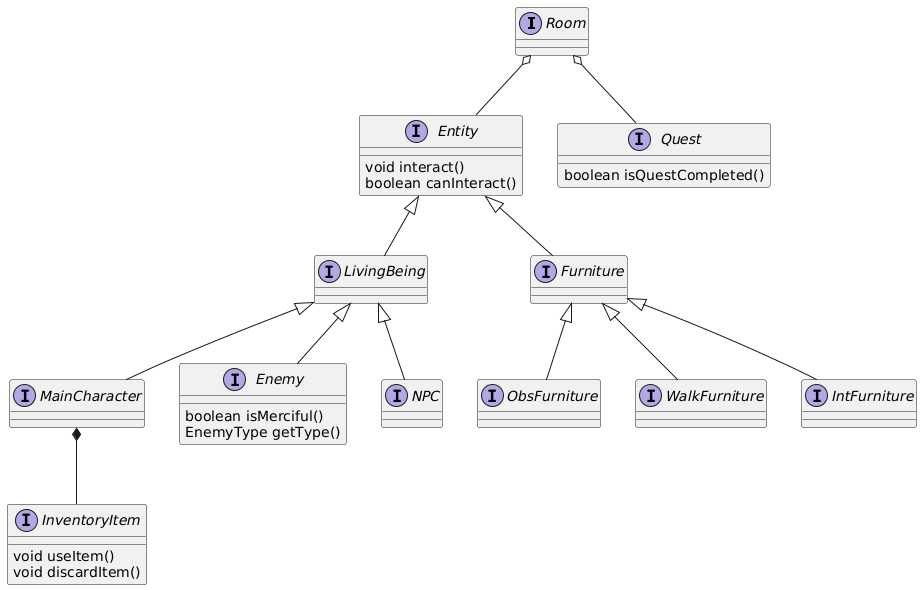
\includegraphics[width=\textwidth]{img/model.png}
	\caption{Schema UML del dominio applicativo}
	\label{img:model}
\end{figure}


\chapter{Design}

\section{Architettura}

Il software si basa sull’architettura MVC nella sua declinazione standard. In particolare, ogni elemento dell’architettura offre un unico entry point verso l’esterno, in modo che gli accessi alle sue funzionalità possano essere uniformi e consistenti, offrendo un ulteriore grado di incapsulamento.
%
\newline Il Model offre come proprio entry point l’interfaccia Room, che fa da scenario base per lo svolgimento della fase di esplorazione del gioco. All’interno della stanza infatti, sono presenti tutte le entità, che vengono modificate ad ogni tick del motore fisico tramite un metodo offerto dalla stessa Room, deputata a controllare anche se le singole entità siano in grado di muoversi al suo interno. 
%
\newline Il Controller, che conserva il riferimento alla stanza in cui attualmente si trova il gioco, gestisce al suo interno le transizioni di stato per le varie fasi del gameplay, interrogando la View per mostrare le interfacce corrette e richiedendo al Model eventuali modifiche. Il Controller è anche responsabile della temporizzazione dell’aggiornamento del motore di gioco, e della traduzione delle entità del Model in elementi rappresentabili correttamente dalla View.
%
\newline La View offre un entry point centrale da cui è possibile richiedere di mostrare le varie interfacce, o l’accesso ai loro riferimenti per chiamare procedure proprie di tali istanze. Nell’architettura realizzata, la View agisce come elemento passivo ricevendo i dati da mostrare dal Controller tramite opportune interrogazioni. La gestione dell’input permette alla View di comunicare particolari eventi al Controller, che li gestirà e ne rifletterà eventualmente gli effetti sul Model.
%
\newline Nella realizzazione dell’architettura MVC, modificare la View non impatta minimamente il Model, dal momento che è solamente il Controller a dialogare con questa componente. Dall’altro lato, il Controller potrebbe essere impattato da una modifica della View radicale (come per esempio trasformare la GUI attiva in un’interfaccia reattiva, oppure la rimozione dei suoni), mentre non sarebbe impattato da modifiche nelle tecniche implementative della GUI - come per esempio una modifica della libreria grafica - a patto che sia in grado di rispettare il contratto stabilito dalle due interfacce (ad esempio accettare gli stessi tipi di chiamate parametrizzate).


\begin{figure}[H]
	\centering{}
	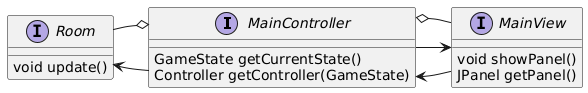
\includegraphics[width=\textwidth]{img/mvc.png}
	\caption{Schema UML degli entry point dei rapporti fra componenti di MVC}
	\label{img:mvc}
\end{figure}

\section{Design dettagliato}

\subsection*{Mazuru Mihai}
//magari introduzione dove dico tutto quello che ho fatto

\section{Furniture}
\textbf{Problema}: Nella modellazione degli oggetti di arredo mi sono imbattuto nel problema 
di come realizzare diverse tipologie di arredi senza ripetizioni di codice. Questi oggetti 
sono caratterizzati da un nome, una descrizione, una posizione e un tipo, e invece si differenziano 
per le seguenti proprietà: attraversabilità e interattività.

\textbf{Soluzione}: Ho optato per l'implementazione del pattern \textit{Template Method}. 
L'ho applicato realizzando una classe astratta \textit{Furniture} che contiene la logica comune a 
tutti gli oggetti di arredo (con i corrispettivi getter) e i metodi astratti \textit{isWalkable()} e 
\textit{isInteractive()}. L'implementazione di questi metodi viene lasciata ad ogni sottoclasse.
Difatti la classe \textit{WalkableFurniture} definisce oggetti di arredo con i quali si può interagire e
che non ostacolano il passaggio delle entità viventi, mentre la classe \textit{ObstructingFurniture} 
definisce oggetti con caratteristiche diametralmente opposte (bloccanti e non interattivi) e 
invece la classe \textit{InteractiveFurniture} definisce oggetti con caratteristiche intermedie(bloccanti ed interattivi).

\newline La soluzione scelta consente inoltre l'estendibilità, facilitando la creazione di una nuova
ipotetica classe con oggetti attraversabili e non interattivi.

\begin{figure}[H]
	\centering{}
	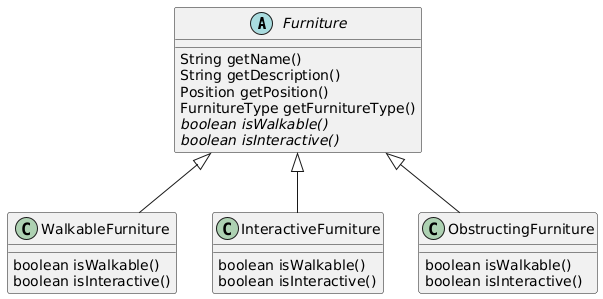
\includegraphics[width=\textwidth]{img/template.png}
	\caption{Schema UML dell'applicazione del pattern Template Method alla gerarchia delle Furniture.}
	\label{img:template}
\end{figure}

\textbf{Problema}:La creazione dei diversi oggetti di arredo attraverso una semplice "new" comporterebbe
l'aggiunta di dipendenze al nostro codice, rendendolo più difficile e tedioso da testare, 
complicando la sua estendibilità ed eventualmente la sua manuntenzione. 

\textbf{Soluzione}:Proprio per questo ho scelto di utilizzare il pattern \textit{Simple Factory} per la 
creazione degli arredi. Ho realizzato un'interfaccia che contiene i metodi per la creazione dei diversi
tipi di arredi. Questi metodi vengono implementati dalla sua sottoclasse, il quale è in grado di creare 
oggetti randomici, specifici oppure solo di un determinato tipo. Gli unici parametri richiesti sono il tipo
e la posizione dell'arredo, mentre le altre caratterische come il nome e la descrizione vengono gestite
internamente alla factory attraverso una mappa che contiene per ogni tipo diverso di arredo una descrizione unica.

\begin{figure}[H]
	\centering{}
	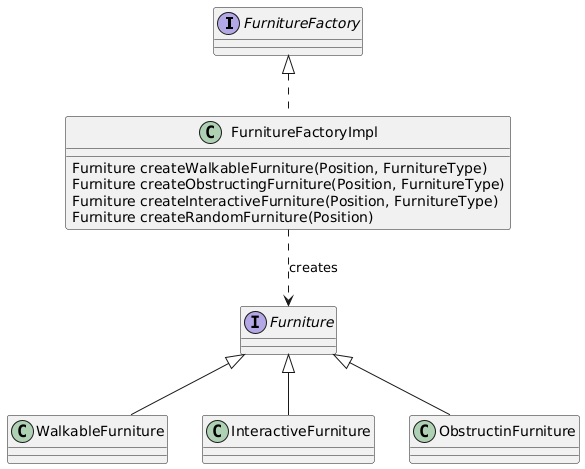
\includegraphics[width=\textwidth]{img/furnitureSimpleFactory.png}
	\caption{Schema UML dell'applicazione del patter Simple Factory per la creazione di Furniture.}
	\label{img:furnitureSimpleFactory}
\end{figure}

\section{Gestione panelli di gioco}

\textbf{Problema}:Il nostro progetto si articola in diversi momenti di gioco e il problema iniziale
era proprio quello di capire come gestire nel migliore dei modi il passaggio da una pannello di gioco ad 
un altro.

\textbf{Soluzione}:Per risolvere questo problema il gruppo ha scelto di creare una \textit{MainView} che
si sarebbe occupata della creazione del frame, della creazione dei vari pannelli di gioco e
delle transizione da un pannello all'altro.
Io mi sono occupato dell'implementazione e ho optato per l'utilizzo di \textit{CardLayout}, un manager layout
che permette di associare ad ogni pannello una stringa di testo, attraverso la quale sarà possibile far emergere
dalla "pila di carte" il pannello desiderato. L'invocazione del metodo per emergere un certo pannello viene effettuata
dal corrispondente controller.
\begin{figure}[H]
	\centering{}
	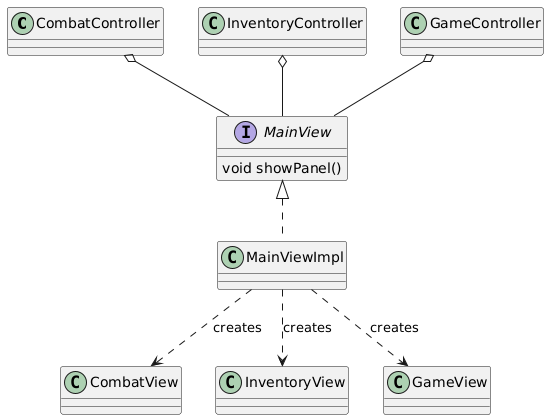
\includegraphics[width=\textwidth]{img/mainView.png}
	\caption{Schema UML che rappresenta MainView, alcuni pannelli di gioco, alcuni controller del gioco e le loro interazioni.}
	\label{img:mainView}
\end{figure}

\section{Gestione combattimento}

\textbf{Problema}:Il combattimento è uno dei momenti di gioco più importanti e la sua gestione  

\textbf{Soluzione}:

\chapter{Sviluppo}
\section{Testing automatizzato}

Per quanto riguarda il testing automatizzato, si è sfruttata la libreria JUnit e si sono realizzati test su quasi tutte le classi di Model e Controller. Ciò è stato fatto per garantire il corretto funzionamento dell’applicazione, e per avere la certezza che gli eventuali problemi riscontrati durante il gioco non fossero dovuti a mancanze di logica implementativa, quanto a problematiche di visualizzazione. 
%
\newline La View, invece, è stata testata manualmente in fase di sviluppo, e poi in fase di collaudo del software, perché personalmente non siamo riusciti ad approfondire le dinamiche di testing automatizzato che avrebbero permesso di testare automaticamente anche quella parte del software.
%
\newline In linea generale, gli aspetti su cui il testing si è maggiormente soffermato sono stati i seguenti:

\begin{itemize}
	\item Generazione della mappa, movimento e interazioni al suo interno. Particolarmente, si è verificato che il movimento e le interazioni non generassero comportamenti imprevisti e che si riflettessero correttamente sugli aggiornamenti del Model.
	\item Combattimento. In particolare, il testing si concentra sul mantenimento dell’ordine dei turni per evitare comportamenti imprevisti, e sul corretto inserimento in inventario del bottino dei nemici sconfitti.
	\item Protagonista. In particolare, si è testato il sistema di gestione della vita del protagonista, così come del suo inventario. Nei controlli sull’inventario, si è verificato il corretto utilizzo degli oggetti curativi, così come delle armi e armature, per garantire comportamenti consistenti in fase di combattimento.
	\item Input utente. Si sono testati i Controller che svolgono la funzione di Observer, per garantire la corretta gestione degli input.
	\item Creazione delle istanze. Avendo fatto largo uso del Pattern Factory, si è deciso di testare i metodi di generazione degli oggetti per verificare l’effettiva consistenza delle istanze create e garantire prevedibilità in fase di gioco.
\end{itemize}

\section{Note di sviluppo}

Questa sezione, come quella riguardante il design dettagliato va svolta \textbf{singolarmente da ogni membro del gruppo}.
%
Nella prima parte, ciascuno dovrà mostrare degli esempi di codice particolarmente ben realizzati,
che dimostrino proefficienza con funzionalità avanzate del linguaggio e capacità di spingersi oltre le librerie mostrate a lezione.

\begin{itemize}
	\item \textbf{Elencare} (fare un semplice elenco per punti, non un testo!) le feature \textit{avanzate} del linguaggio e dell'ecosistema Java che sono state
utilizzate. Le feature di interesse sono:
	\begin{itemize}
		\item Progettazione con generici, ad esempio costruzione di nuovi tipi generici, e uso di generici bounded.
		L'uso di classi generiche di libreria non è considerato avanzato.
		\item Uso di lambda expressions
		\item Uso di \texttt{Stream}, di \texttt{Optional} o di altri costrutti funzionali
		\item Uso di reflection
		\item Definizione ed uso di nuove annotazioni
		\item Uso del Java Platform Module System
		\item Uso di parti della libreria JDK non spiegate a lezione (networking, compressione, parsing XML, eccetera...)
		\item Uso di librerie di terze parti (incluso JavaFX): Google Guava, Apache Commons...
	\end{itemize}
	\item Si faccia molta attenzione a non scrivere banalità, elencando qui features di tipo ``core'', come le eccezioni, le enumerazioni, o le inner class: nessuna di queste è considerata avanzata.
	\item Per ogni feature avanzata, mostrata, includere:
	\begin{itemize}
		\item Nome della feature
		\item Permalink GitHub al punto nel codice in cui è stata utilizzata
	\end{itemize}
\end{itemize}

In questa sezione, \textit{dopo l'elenco},
vanno menzionati ed attributi con precisione eventuali pezzi di codice ``riadattati'' (o scopiazzati...) da Internet o da altri progetti,
pratica che tolleriamo ma che non raccomandiamo.
%
Si rammenta agli studenti che non è consentito partire da progetti esistenti e procedere per modifiche successive.
%
Si ricorda anche che i docenti hanno in mano strumenti antiplagio piuttosto raffinati e che ``capiscono'' il codice e la storia delle modifiche del progetto,
per cui tecniche banali come cambiare nomi (di classi, metodi, campi, parametri, o variabili locali),
aggiungere o togliere commenti,
oppure riordinare i membri di una classe vengono individuate senza problemi.
%
Le regole del progetto spiegano in dettaglio l'approccio dei docenti verso atti gravi come il plagiarismo.

I pattern di design \textbf{non} vanno messi qui.
%
L'uso di pattern di design (come suggerisce il nome) è un aspetto avanzato di design, non di implementazione,
e non va in questa sezione.

\subsection*{Elementi positivi}

\begin{itemize}
	\item Si elencano gli aspetti avanzati di linguaggio che sono stati impiegati
	\item Si elencano le librerie che sono state utilizzate
	\item Per ciascun elemento, si fornisce un permalink
	\item Ogni permalink fa riferimento ad uno snippet di codice scritto dall'autore della sezione (i docenti verificheranno usando \texttt{git blame})
	\item Se si è utilizzato un particolare algoritmo, se ne cita la fonte originale.
	Ad esempio, se si è usato Mersenne Twister per la generazione di numeri pseudo-random, si cita \cite{mersenne}.
	\item Si identificano parti di codice prese da altri progetti, dal web, o comunque scritte in forma originale da altre persone.
	In tal senso, si ricorda che agli ingegneri non è richiesto di re-inventare la ruota continuamente:
	se si cita debitamente la sorgente è tollerato fare uso di di snippet di codice open source per risolvere velocemente problemi non banali.
	Nel caso in cui si usino snippet di codice di qualità discutibile,
	oltre a menzionarne l'autore originale si invitano gli studenti ad adeguare tali parti di codice agli standard e allo stile del progetto.
	Contestualmente, si fa presente che è largamente meglio fare uso di una libreria che copiarsi pezzi di codice:
	qualora vi sia scelta (e tipicamente c'è), si preferisca la prima via.
\end{itemize}

\subsection*{Elementi negativi}
\begin{itemize}
	\item Si elencano feature core del linguaggio invece di quelle segnalate. Esempi di feature core da non menzionare sono:
    \begin{itemize}
        \item eccezioni;
        \item classi innestate;
        \item enumerazioni;
        \item interfacce.
    \end{itemize}
	\item Si elencano applicazioni di terze parti (peggio se per usarle occorre licenza, e lo studente ne è sprovvisto) che non c'entrano nulla con lo sviluppo, ad esempio:
    \begin{itemize}
        \item Editor di grafica vettoriale come Inkscape o Adobe Illustrator;
        \item Editor di grafica scalare come GIMP o Adobe Photoshop;
        \item Editor di audio come Audacity;
        \item Strumenti di design dell'interfaccia grafica come SceneBuilder: il codice è in ogni caso inteso come sviluppato da voi.
    \end{itemize}
	\item Si descrivono aspetti di scarsa rilevanza, o si scende in dettagli inutili.
	\item Sono presenti parti di codice sviluppate originalmente da altri che non vengono debitamente segnalate.
	In tal senso, si ricorda agli studenti che i docenti hanno accesso a tutti i progetti degli anni passati,
	a Stack Overflow,
	ai principali blog di sviluppatori ed esperti Java,
	ai blog dedicati allo sviluppo di soluzioni e applicazioni
	(inclusi blog dedicati ad Android e allo sviluppo di videogame),
	nonché ai vari GitHub, GitLab, e Bitbucket.
	Conseguentemente, è \emph{molto} conveniente \emph{citare} una fonte ed usarla invece di tentare di spacciare per proprio il lavoro di altri.
	\item Si elencano design pattern
\end{itemize}

\subsection{Esempio}

\subsubsection{Utilizzo della libreria SLF4J}

Utilizzata in vari punti.
Un esempio è \url{https://github.com/AlchemistSimulator/Alchemist/blob/5c17f8b76920c78d955d478864ac1f11508ed9ad/alchemist-swingui/src/main/java/it/unibo/alchemist/boundary/swingui/effect/impl/EffectBuilder.java#L49}

\subsubsection{Utilizzo di \texttt{LoadingCache} dalla libreria Google Guava}

Permalink: \url{https://github.com/AlchemistSimulator/Alchemist/blob/d8a1799027d7d685569e15316a32e6394632ce71/alchemist-incarnation-protelis/src/main/java/it/unibo/alchemist/protelis/AlchemistExecutionContext.java#L141-L143}

\subsubsection{Utilizzo di \texttt{Stream} e lambda expressions}

Usate pervasivamente. Il seguente è un singolo esempio.
Permalink: \url{https://github.com/AlchemistSimulator/Alchemist/blob/d8a1799027d7d685569e15316a32e6394632ce71/alchemist-incarnation-protelis/src/main/java/it/unibo/alchemist/model/ProtelisIncarnation.java#L98-L120}

\subsubsection{Scrittura di metodo generico con parametri contravarianti}

Permalink: \url{https://github.com/AlchemistSimulator/Alchemist/blob/d8a1799027d7d685569e15316a32e6394632ce71/alchemist-incarnation-protelis/src/main/java/it/unibo/alchemist/protelis/AlchemistExecutionContext.java#L141-L143}

\subsubsection{Protezione da corse critiche usando \texttt{Semaphore}}

Permalink: \url{https://github.com/AlchemistSimulator/Alchemist/blob/d8a1799027d7d685569e15316a32e6394632ce71/alchemist-incarnation-protelis/src/main/java/it/unibo/alchemist/model/ProtelisIncarnation.java#L388-L440}


\chapter{Commenti finali}

In quest'ultimo capitolo si tirano le somme del lavoro svolto e si delineano eventuali sviluppi
futuri.

\textit{Nessuna delle informazioni incluse in questo capitolo verrà utilizzata per formulare la valutazione finale}, a meno che non sia assente o manchino delle sezioni obbligatorie.
%
Al fine di evitare pregiudizi involontari, l'intero capitolo verrà letto dai docenti solo dopo aver formulato la valutazione.

\section{Autovalutazione e lavori futuri}

\textbf{È richiesta una sezione per ciascun membro del gruppo, obbligatoriamente}.
%
Ciascuno dovrà autovalutare il proprio lavoro, elencando i punti di forza e di debolezza in quanto prodotto.
Si dovrà anche cercare di descrivere \emph{in modo quanto più obiettivo possibile} il proprio ruolo all'interno del gruppo.
Si ricorda, a tal proposito, che ciascuno studente è responsabile solo della propria sezione: non è un problema se ci sono opinioni contrastanti, a patto che rispecchino effettivamente l'opinione di chi le scrive.
Nel caso in cui si pensasse di portare avanti il progetto, ad esempio perché effettivamente impiegato, o perché sufficientemente ben riuscito da poter esser usato come dimostrazione di esser capaci progettisti, si descriva brevemente verso che direzione portarlo.

\section{Difficoltà incontrate e commenti per i docenti}

Questa sezione, \textbf{opzionale}, può essere utilizzata per segnalare ai docenti eventuali problemi o difficoltà incontrate nel corso o nello svolgimento del progetto, può essere vista come una seconda possibilità di valutare il corso (dopo quella offerta dalle rilevazioni della didattica) avendo anche conoscenza delle modalità e delle difficoltà collegate all'esame, cosa impossibile da fare usando le valutazioni in aula per ovvie ragioni.
%
È possibile che alcuni dei commenti forniti vengano utilizzati per migliorare il corso in futuro: sebbene non andrà a vostro beneficio, potreste fare un favore ai vostri futuri colleghi.
%
Ovviamente \textit{il contenuto della sezione non impatterà il voto finale}.

\appendix
\chapter{Guida utente}

Capitolo in cui si spiega come utilizzare il software. Nel caso in cui il suo uso sia del tutto
banale, tale capitolo può essere omesso.
%
A tal riguardo, si fa presente agli studenti che i docenti non hanno mai utilizzato il software
prima, per cui aspetti che sembrano del tutto banali a chi ha sviluppato l'applicazione possono non
esserlo per chi la usa per la prima volta.
%
Se, ad esempio, per cominciare una partita con un videogioco è necessario premere la barra
spaziatrice, o il tasto ``P'', è necessario che gli studenti lo segnalino.

\subsection*{Elementi positivi}

\begin{itemize}
 \item Si istruisce in modo semplice l'utente sull'uso dell'applicazione, eventualmente facendo uso di schermate e descrizioni.
\end{itemize}

\subsection*{Elementi negativi}
\begin{itemize}
 \item Si descrivono in modo eccessivamente minuzioso tutte le caratteristiche, anche minori, del software in oggetto.
 \item Manca una descrizione che consenta ad un utente qualunque di utilizzare almeno le funzionalità primarie dell'applicativo.
\end{itemize}

\chapter{Esercitazioni di laboratorio}

In questo capitolo ciascuno studente elenca gli esercizi di laboratorio che ha svolto
(se ne ha svolti),
elencando i permalink dei post sul forum dove è avvenuta la consegna.
%
Questa sezione potrebbe essere processata da strumenti automatici,
per cui link a oggetti diversi dal permalink della consegna,
errori nell'email o nel nome del laboratorio possono portare ad ignorare alcune consegne,
si raccomanda la massima precisione.

\section*{Esempio}

\subsection{paolino.paperino@studio.unibo.it}

\begin{itemize}
 \item Laboratorio 04: \url{https://virtuale.unibo.it/mod/forum/discuss.php?d=12345#p123456}
 \item Laboratorio 06: \url{https://virtuale.unibo.it/mod/forum/discuss.php?d=22222#p222222}
 \item Laboratorio 09: \url{https://virtuale.unibo.it/mod/forum/discuss.php?d=99999#p999999}
\end{itemize}

\subsection{paperon.depaperoni@studio.unibo.it}

\begin{itemize}
 \item Laboratorio 04: \url{https://virtuale.unibo.it/mod/forum/discuss.php?d=12345#p123456}
 \item Laboratorio 05: \url{https://virtuale.unibo.it/mod/forum/discuss.php?d=22222#p222222}
 \item Laboratorio 06: \url{https://virtuale.unibo.it/mod/forum/discuss.php?d=99999#p999999}
 \item Laboratorio 07: \url{https://virtuale.unibo.it/mod/forum/discuss.php?d=22222#p222222}
 \item Laboratorio 08: \url{https://virtuale.unibo.it/mod/forum/discuss.php?d=99999#p999999}
 \item Laboratorio 09: \url{https://virtuale.unibo.it/mod/forum/discuss.php?d=22222#p222222}
 \item Laboratorio 10: \url{https://virtuale.unibo.it/mod/forum/discuss.php?d=99999#p999999}
 \item Laboratorio 11: \url{https://virtuale.unibo.it/mod/forum/discuss.php?d=22222#p222222}
\end{itemize}


\bibliographystyle{alpha}
\bibliography{13-template}

\end{document}
